\documentclass[a4paper,10pt]{article}

\usepackage[utf8x]{inputenc}
\usepackage{makeidx}
\usepackage{listings}
\usepackage{color}
\usepackage{graphicx}
\usepackage{hyperref}

%\usepackage{html}   %  *always* load this for LaTeX2HTML
%\begin{htmlonly}
%  \usepackage{verbatim}
%  \providecommand{\lstlisting}[2][]{\verbatiminput{#2}}
%\end{htmlonly}

\input colordvi
\definecolor{lightblue}{rgb}{.3,.5,1}
\definecolor{orange}{rgb}{1,.7,0}
\definecolor{darkorange}{rgb}{1,.4,0}
\definecolor{darkgreen}{rgb}{0,.4,0}
\definecolor{darkblue}{rgb}{0,0,.4}
\definecolor{darkred}{rgb}{.56,0,0}
\definecolor{gray}{rgb}{.3,.3,.3}
\definecolor{darkgray}{rgb}{.2,.2,.2}
\definecolor{shadecolor}{gray}{0.925}

\lstdefinelanguage{GEXF}{
    morekeywords=[0]{gexf, meta, graph, creator, description, nodes, edges, node, edge, attributes, attribute, options, attvalues, attvalue, default, keywords, color, size, position, shape, thickness, parents, parent, spells, spell, viz},
    morekeywords=[1]{id, for, pid, label, source, target, mode, defaultedgetype, type, lastmodifieddate, start, startopen, end, endopen, timetype, cardinal, class, count, title, value, r, g, b, x, y, z, a, xmlns},
    morekeywords=[2]{simple, double, static, dynamic, integer, double, float, boolean, liststring, string, date, anyURI},
    morestring=[b]",
}

\lstdefinestyle{gexf}{
    language=GEXF,
    xleftmargin=\parindent,
    xrightmargin=\parindent,
    aboveskip=3mm,
    belowskip=3mm,
    tabsize=2,
    columns=[l]fullflexible,
    showstringspaces=false,
    % text styles
    basicstyle=\scriptsize\ttfamily,
    commentstyle=\footnotesize\rmfamily\em,
    stringstyle=\rmfamily\em\color{gray},
    keywordstyle=[0]\color{blue},
    keywordstyle=[1]\color{darkorange},
    keywordstyle=[2]\underbar,
    % numbers
    numbers=left,
    numberstyle=\tiny,
    stepnumber=3,
    firstnumber=1,
    % decoration
    frame=shadowbox,
    frameround=tttf
    %backgroundcolor=\color{shadecolor}
}

\lstdefinelanguage{RNC}{
    morekeywords=[1]{start,element,attribute,text,empty,string,text},
    morekeywords=[2]{default,namespace,datatypes},
    morekeywords=[3]{grammar,include,parent,inherit},
    morekeywords=[4]{xsd},
    morekeywords=[5]{a,defaultValue},
    morestring=[b]",
    morecomment=[l]{\#},
    alsodigit={-},
    sensitive
}


\lstdefinestyle{rnc}{
    language=RNC,
    basicstyle=\scriptsize\ttfamily,
    commentstyle=\footnotesize\sffamily\em\color{darkgreen},
    stringstyle=\sffamily\color{red},
    keywordstyle=[1]\color{blue}\bfseries,
    keywordstyle=[2]\color{lightblue}\bfseries,
    keywordstyle=[3]\color{lightblue}\bfseries,
    keywordstyle=[4]\color{darkgreen}\bfseries,
    keywordstyle=[5]\color{orange}\bfseries
}

%\lstdefinestyle{xml}{
    language=XML,
    xleftmargin=\parindent,
    xrightmargin=\parindent,
    aboveskip=3mm,
    belowskip=3mm,
    basicstyle=\footnotesize\ttfamily,
    commentstyle=\small\rmfamily\em,
    tabsize=2,
    columns=[l]fullflexible,
    showstringspaces=false,
    % keywords
    keywordstyle=\color{blue}\bfseries,
    stringstyle=\color{red},
    usekeywordsintag=false,
    markfirstintag=true,
    % numbers
    numbers=left,
    numberstyle=\tiny,
    stepnumber=3,
    firstnumber=1,
    % decoration
    frame=shadowbox,
    frameround=tttf,
    backgroundcolor=\color{shadecolor}
}


\hypersetup{
    bookmarks=true,         % show bookmarks bar?
    unicode=false,          % non-Latin characters in Acrobat’s bookmarks
    pdftoolbar=true,        % show Acrobat’s toolbar?
    pdfmenubar=true,        % show Acrobat’s menu?
    pdffitwindow=false,     % window fit to page when opened
    pdfstartview={FitH},    % fits the width of the page to the window
    pdftitle={GEXF 1.2draft Primer},    % title
    pdfauthor={Sebastien Heymann},     % author
    pdfsubject={GEXF 1.2draft Primer},   % subject of the document
    pdfcreator={Gephi},   % creator of the document
    pdfproducer={Gephi}, % producer of the document
    pdfkeywords={gephi gexf graph}, % list of keywords
    pdfnewwindow=true,      % links in new window
    colorlinks=false,       % false: boxed links; true: colored links
    linkcolor=red,          % color of internal links
    citecolor=green,        % color of links to bibliography
    filecolor=magenta,      % color of file links
    urlcolor=cyan           % color of external links
}

\makeindex


%opening
\title{GEXF 1.2draft Primer}
\author{GEXF Working Group}

\begin{document}

\maketitle

\begin{abstract}
GEXF Primer is a non-normative document intended to provide an easily readable description of the GEXF facilities, and is oriented towards quickly understanding how to create GEXF documents. This primer describes the language features through examples which are complemented by references to normative texts. Specification is in \href{http://relaxng.org/compact-tutorial-20030326.html}{RelaxNG Compact} grammar.
\end{abstract}

\tableofcontents

\section{Introduction} \label{introduction}

\paragraph{}
This document, GEXF Primer, provides an description of GEXF, and should be used alongside the formal descriptions of the language contained in the GEXF specification. The intended audience of this document includes application developers whose programs read and write GEXF files, and users who want to communicate with programs using GEXF import/export. The text assumes that you have a basic understanding of XML 1.0 and  XML-Namespaces. Basic knowledge of XML Schema is also assumed for some parts of this document. Each major section of the primer introduces new features of the language, and describes those features in the context of concrete examples.

Section 2 covers the basic mechanisms of GEXF. It describes how to declare a simple graph by defining its nodes and edges and how to add simple user data to the graph.

Section 3 describes dynamic graph model.

Section 4 describes mechanisms for extending GEXF to add specific data with the Visualization module in example.

\paragraph{}
The primer is a non-normative document, which means that it does not provide a definitive specification of the GEXF language. The examples and other explanatory material in this document are provided to help you understand GEXF, but they may not always provide definitive answers. In such cases, you will need to refer to the GEXF specification, and to help you do this, we provide many links pointing to the relevant parts of the specification.

\section{Basic Concepts} \label{basic}

The purpose of a GEXF document is to define a graph representing a network. Let us start by considering the minimal graph shown in the figure below. It contains 2 nodes and 1 edge.

\begin{figure}[!ht]
  \begin{center}
  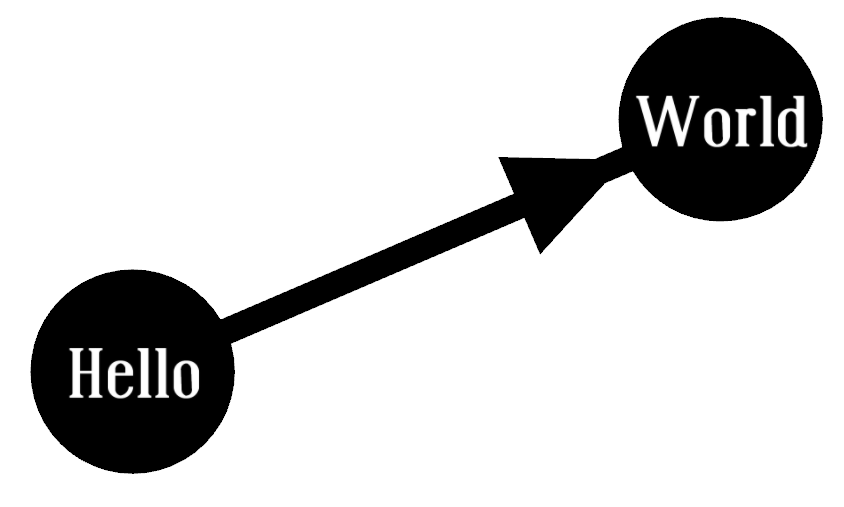
\includegraphics[scale=0.15]{res/simple.png}
  \caption{Hello-world graph}
  \end{center}
\end{figure}

\subsection{A Simple Graph}

This is a dummy graph:

\lstset{ style=gexf }
\begin{lstlisting}[caption={Hello world!},label=helloworld]
<?xml version="1.0" encoding="UTF-8"?>
<gexf xmlns="http://www.gexf.net/1.2draft"
       xmlns:xsi="http://www.w3.org/2001/XMLSchema-instance"
       xsi:schemaLocation="http://www.gexf.net/1.2draft
                             http://www.gexf.net/1.2draft/gexf.xsd"
      version="1.2">
  <meta lastmodifieddate="2009-03-20">
    <creator>Gephi.org</creator>
    <description>A hello world! file</description>
  </meta>
  <graph defaultedgetype="directed">
    <nodes>
      <node id="0" label="Hello"/>
      <node id="1" label="Word"/>
    </nodes>
    <edges>
      <edge id="0" source="0" target="1"/>
    </edges>
  </graph>
</gexf>
\end{lstlisting}

The GEXF document consists of a gexf element and a variety of subelements: graph, node, edge. In the remainder of this section we will discuss these elements in detail and show how they define a graph.

\subsection{Header}

In this section we discuss the parts of the document which are common to all GEXF documents, basically the gexf element and the meta declaration.

\lstset{ style=gexf }
\begin{lstlisting}[caption={Header},label=header]
<?xml version="1.0" encoding="UTF-8"?>
<gexf xmlns="http://www.gexf.net/1.2draft"
       xmlns:xsi="http://www.w3.org/2001/XMLSchema-instance"
       xsi:schemaLocation="http://www.gexf.net/1.2draft
                             http://www.gexf.net/1.2draft/gexf.xsd"
      version="1.2">
  <meta lastmodifieddate="2009-03-20">
    <creator>Gephi.org</creator>
    <description>A hello world! file</description>
    <keywords>basic, web</keywords>
  </meta>
  ...
</gexf>
\end{lstlisting}

\paragraph{}
The first line of the document is an XML process instruction which defines that the document adheres to the XML 1.0 standard and that the encoding of the document is UTF-8, the standard encoding for XML documents. Of course other encodings can be chosen for GEXF documents.

\paragraph{}
The second line contains the root-element element of a GEXF document: the gexf element. The gexf element, like all other GEXF elements, belongs to the namespace \begin{footnotesize}http://www.gexf.net/1.2draft\end{footnotesize}. For this reason we define this namespace as the default namespace in the document by adding the XML Attribute \begin{footnotesize}xmlns="http://www.gexf.net/1.2draft"\end{footnotesize} to it. The two other XML Attributes are needed to specify the XML Schema for this document. In our example we use the standard schema for GEXF documents located on the gexf.net server. The first attribute, \begin{footnotesize}xmlns:xsi="http://www.w3.org/2001/XMLSchema-instance"\end{footnotesize}, defines xsi as the XML Schema namespace. The second attribute, \begin{footnotesize}xsi:schemaLocation ="http://www.gexf.net/1.2draft http://www.gexf.net/1.2draft/gexf.xsd"\end{footnotesize}, defines the XML Schema location for all elements in the GEXF namespace.

\paragraph{}
The XML Schema reference is not required but it provides means to validate the document and is therefore strongly recommended.

\paragraph{}
The \begin{footnotesize}meta\end{footnotesize} element contains additionnal information about the network. Element leafs are assumed to be text, and \begin{footnotesize}lastmodifieddate\end{footnotesize} is an international standard date (yyyy-mm-dd). The \begin{footnotesize}graph\end{footnotesize} element must be declared after the \begin{footnotesize}meta\end{footnotesize} element.

\paragraph{}
GEXF document is specified in the \href{http://relaxng.org/compact-tutorial-20030326.html}{RelaxNG Compact} file \href{http://www.gexf.net/1.2draft/gexf.rnc}{gexf.rc}. Header is ruled by the following declaration :

\lstset{ style=rnc }
\begin{lstlisting}[caption={Header Specification},label=headerRNC]
default namespace = "http://www.gexf.net/1.2draft"
namespace     rng = "http://relaxng.org/ns/structure/1.0"
datatypes     xsd = "http://www.w3.org/2001/XMLSchema-datatypes"

# Grammar root
start = element gexf { gexf-content }

# Tree
gexf-content =
    attribute version { string "1.2" }
  & attribute variant { xsd:string }?
  & (element meta { meta-content }?
  ,  element graph { graph-content })

# Attributes & Leafs
meta-content =
    attribute lastmodifieddate { xsd:date }?
  & element creator { text }?
  & element keywords { text }?
  & element description { text }?
\end{lstlisting}

\subsection{Network Topology} \label{networktopology}

The network topology structure containing nodes and edges is called the graph. A graph is, not surprisingly, denoted by a \begin{footnotesize}graph\end{footnotesize} element. Nested inside a graph element are the declarations of nodes and edges. A node is declared with the \begin{footnotesize}node\end{footnotesize} element inside a \begin{footnotesize}nodes\end{footnotesize} element, and an egde with the \begin{footnotesize}edge\end{footnotesize} element inside an \begin{footnotesize}edges\end{footnotesize} element. Nodes and edges order doesn't matter.

\lstset{ style=gexf }
\begin{lstlisting}[caption={The definition of the graph},label=topology]
<graph defaultedgetype="directed">
  <nodes>
    <node id="0" label="Hello" />
    <node id="1" label="Word" />
    ...
  </nodes>
  <edges>
    <edge id="0" source="0" target="1" weight="3.167" />
    ...
  </edges>
</graph>
\end{lstlisting}

\subsubsection{Declaring a Graph}

Graphs in GEXF are mixed, in other words, they can contain directed and undirected edges at the same time. If no direction is specified when an edge is declared, the default direction \begin{footnotesize}defaultedgetype\end{footnotesize} is applied to the edge. If you know what kind of edges are stored, you may interpret the mixed graph as a directed or an undirected graph at your own risks.

The default direction is declared as the optional XML-attribute \begin{footnotesize}defaultedgetype\end{footnotesize} of the \begin{footnotesize}graph\end{footnotesize} element. The three possible values for this XML-attribute are \textit{directed}, \textit{undirected} and \textit{mutual}. Note that the default direction is optional and would be assumed as \textit{undirected}.

The optional XML-attribute \begin{footnotesize}mode\end{footnotesize} set the kind of network: static or dynamic. Last one provides time support (see  the section \ref{dynamics} on Dynamics). Static mode is assumed by default.

The \begin{footnotesize}edges\end{footnotesize} element must be declared after the \begin{footnotesize}nodes\end{footnotesize} element.

\lstset{ style=gexf }
\begin{lstlisting}[caption={An empty graph!},label=aGraph]
<graph>
  <nodes>
  </nodes>
  <edges>
  </edges>
</graph>
\end{lstlisting}

\lstset{ style=rnc }
\begin{lstlisting}[caption={Topology Specification},label=topologyRNC]
graph-content =
    attribute defaultedgetype { defaultedgetype-type }?
  & attribute idtype { idtype-type }?
  & attribute mode { mode-type }?
  & (element nodes { nodes-content }
  ,  element edges { edges-content })


# Nodes

nodes-content =
    attribute count { xsd:nonNegativeInteger }?
  & element node { node-content }*

node-content =
    attribute id { id-type }
  & attribute label { xsd:token }?


# Edges

edges-content =
    attribute count { xsd:nonNegativeInteger }?
  & element edge { edge-content }*

edge-content =
    attribute id { id-type }
  & attribute type { edgetype-type }?
  & attribute label { xsd:token }?
  & attribute source { id-type }
  & attribute target { id-type }
  & attribute weight { weight-type }?


# Datatypes

defaultedgetype-type = [ a:defaultValue = "undirected" ]
    string "directed" |
    string "undirected" |
    string "mutual"

edgetype-type = [ a:defaultValue = "undirected" ]
    string "directed" |
    string "undirected" |
    string "mutual"

id-type =
    xsd:string | xsd:integer

idtype-type = [ a:defaultValue = "string" ]
    string "integer" |
    string "string"

mode-type = [ a:defaultValue = "static" ]
    string "static" |
    string "dynamic"

weight-type = [ a:defaultValue = "1.0" ]
    xsd:float
\end{lstlisting}

\subsubsection{Declaring a Node}

Nodes in the graph are declared by the \begin{footnotesize}node\end{footnotesize} element. Each node has an identifier, which must be unique within the entire document, i.e., in a document there must be no two nodes with the same identifier. The identifier of a node is defined by the XML-attribute \begin{footnotesize}id\end{footnotesize}, which is a string. Each node must have a XML-attribute \begin{footnotesize}label\end{footnotesize}, which is a string.

\lstset{ style=gexf }
\begin{lstlisting}[caption={A node!},label=aNode]
<node id="0" label="Hello world" />
\end{lstlisting}

\lstset{ style=rnc }
\begin{lstlisting}[caption={Node Specification},label=nodeRNC]
node-content =
    attribute id { id-type }
  & attribute label { xsd:token }?

id-type =
    xsd:string | xsd:integer
\end{lstlisting}

\subsubsection{Declaring an Edge}

Edges in the graph are declared by the \begin{footnotesize}edge\end{footnotesize} element. Each edge must define its two endpoints with the XML-Attributes \begin{footnotesize}source\end{footnotesize} and \begin{footnotesize}target\end{footnotesize}. The value of the source, resp. target, must be the identifier of a node in the same document. The identifier of an edge is defined by the XML-Attribute \begin{footnotesize}id\end{footnotesize}. There is no order notion applied to edges.

Edges with only one endpoint, also called loops, selfloops, or reflexive edges, are defined by having the same value for source and target.

Each edge can have a optional XML-attribute \begin{footnotesize}label\end{footnotesize}, which is a string.

The optional XML-attribute \begin{footnotesize}type\end{footnotesize} declares if the edge is \textit{directed}, \textit{undirected} or \textit{mutual} (directed \textit{from source to target and from target to source}). If the direction is not explicitely defined, the default direction is applied to this edge as defined in the enclosing graph.

The weight of the edge is set by the optional XML-attribute \begin{footnotesize}weight\end{footnotesize} and is a float.

Assuming two nodes having respectively the \begin{footnotesize}id\end{footnotesize} value set to \textit{0} and \textit{1}:

\lstset{ style=gexf }
\begin{lstlisting}[caption={An edge!},label=anEdge]
<edge id="0" source="0" target="1"/>
\end{lstlisting}

\lstset{ style=gexf }
\begin{lstlisting}[caption={A more complete edge},label=aMoreEdge]
<edge id="0" source="0" target="1" type="directed" weight="2.4" />
\end{lstlisting}

\lstset{ style=rnc }
\begin{lstlisting}[caption={Edge Specification},label=edgeRNC]
edge-content =
    attribute id { id-type }
  & attribute type { edgetype-type }?
  & attribute label { xsd:token }?
  & attribute source { id-type }
  & attribute target { id-type }
  & attribute weight { weight-type }?

# Datatypes

id-type =
    xsd:string | xsd:integer

edgetype-type = [ a:defaultValue = "undirected" ]
    string "directed" |
    string "undirected" |
    string "mutual"

weight-type = [ a:defaultValue = "1.0" ]
    xsd:float
\end{lstlisting}

\subsection{Network Data} \label{networkdata}

\paragraph{}
In the previous section we discussed how to describe the topology of a graph in GEXF. While pure topological information may be sufficient for some applications, these days focus is made on network analysis based on data attributes. Data are everywhere.

\paragraph{}
A bunch of data can be stored within attributes. The concept is the same as table data or SQL. An attribute has a title/name and a value. Attribute’s name/title must be declared for the whole graph. It could be for instance “degree”, “valid” or “url”. Besides the name of the attribute a column also contains the type.

\subsubsection{Data types}

GEXF uses the XML Schema Data Types (\href{http://www.w3.org/TR/xmlschema-2/}{XSD 1.1}) for the following primitives: \href{http://www.w3.org/TR/xmlschema-2/#string}{string}, \href{http://www.w3.org/TR/xmlschema-2/#decimal}{integer}, \href{http://www.w3.org/TR/xmlschema-2/#float}{float}, \href{http://www.w3.org/TR/xmlschema-2/#double}{double}, \href{http://www.w3.org/TR/xmlschema-2/#boolean}{boolean}, \href{http://www.w3.org/TR/xmlschema-2/#date}{date}, and \href{http://www.w3.org/TR/xmlschema-2/#anyURI}{anyURI}.

\subsubsection{Attributes Example}

Each Node of this graph has three attributes : an url, an indegree value and a boolean for french websites which is set to \textit{true} by default.

\lstset{ style=gexf }
\begin{lstlisting}[caption={A (small) Web Graph},label=webgraph]
<?xml version="1.0" encoding="UTF-8"?>
<gexf xmlns="http://www.gexf.net/1.2draft"
       xmlns:xsi="http://www.w3.org/2001/XMLSchema-instance"
       xsi:schemaLocation="http://www.gexf.net/1.2draft
                             http://www.gexf.net/1.2draft/gexf.xsd"
      version="1.2">
  <meta lastmodifieddate="2009-03-20">
    <creator>Gephi.org</creator>
    <description>A Web network</description>
  </meta>
  <graph defaultedgetype="directed">
    <attributes class="node">
      <attribute id="0" title="url" type="string"/>
      <attribute id="1" title="indegree" type="float"/>
      <attribute id="2" title="frog" type="boolean">
        <default>true</default>
      </attribute>
    </attributes>
    <nodes>
      <node id="0" label="Gephi">
        <attvalues>
          <attvalue for="0" value="http://gephi.org"/>
          <attvalue for="1" value="1"/>
        </attvalues>
      </node>
      <node id="1" label="Webatlas">
        <attvalues>
          <attvalue for="0" value="http://webatlas.fr"/>
          <attvalue for="1" value="2"/>
        </attvalues>
      </node>
      <node id="2" label="RTGI">
        <attvalues>
          <attvalue for="0" value="http://rtgi.fr"/>
          <attvalue for="1" value="1"/>
        </attvalues>
      </node>
      <node id="3" label="BarabasiLab">
        <attvalues>
          <attvalue for="0" value="http://barabasilab.com"/>
          <attvalue for="1" value="1"/>
          <attvalue for="2" value="false"/>
        </attvalues>
      </node>
    </nodes>
    <edges>
      <edge id="0" source="0" target="1"/>
      <edge id="1" source="0" target="2"/>
      <edge id="2" source="1" target="0"/>
      <edge id="3" source="2" target="1"/>
      <edge id="4" source="0" target="3"/>
    </edges>
  </graph>
</gexf>
\end{lstlisting}


\subsubsection{Declaring Attributes}

Attributes are declared inside an \begin{footnotesize}attributes\end{footnotesize} element. The XML-attribute \begin{footnotesize}class\end{footnotesize} apply nested attributes on nodes (\textit{node} value) or edges (\textit{edge} value). You may specify the data type between \textit{integer, double, float, boolean, string and liststring}, and specify a default value.

\lstset{ style=gexf }
\begin{lstlisting}[caption={Attributes Definition},label=attributesDef]
<graph mode="static">
  <attributes class="node">
    <attribute id="0" title="my-text-attribute" type="string"/>
    <attribute id="1" title="my-int-attribute" type="integer"/>
    <attribute id="2" title="my-bool-attribute" type="boolean"/>
  </attributes>
  <attributes class="edge">
    <attribute id="0" title="my-float-attribute" type="float">
      <default>2.0</default>
    </attribute>
  </attributes>
  ...
</graph>
\end{lstlisting}

\lstset{ style=rnc }
\begin{lstlisting}[caption={Attributes Specification},label=attributesRNC]
attributes-content =
    attribute class { class-type }
  & attribute mode { mode-type }?
  & element attribute { attribute-content }*

attribute-content =
    attribute id { id-type }
  & attribute title { xsd:string }
  & attribute type { attrtype-type }
  & element default { text }?
  & element options { text }?


# Datatypes

class-type =
    string "node" |
    string "edge"

mode-type = [ a:defaultValue = "static" ]
    string "static" |
    string "dynamic"

attrtype-type =
    string "integer" |
    string "long" |
    string "double" |
    string "float" |
    string "boolean" |
    string "liststring" |
    string "string" |
    string "anyURI"
\end{lstlisting}

\subsubsection{Defining Attribute Values}

You may understand attributes while looking at this node definition. Besides native fields (id, label), node values are set for three attributes. Omitting an attribute will set the default value as its value. If no default value is set, this is an error.

\lstset{ style=gexf }
\begin{lstlisting}[caption={Node Attributes},label=nodeattributes]
<node id="0" label="Hello world">
  <attvalues>
    <attvalue for="0" value="samplevalue"/>
    <attvalue for="1" value="1831"/>
    <attvalue for="2" value="true"/>
  </attvalues>
</node>
\end{lstlisting}

\lstset{ style=gexf }
\begin{lstlisting}[caption={Edge Attributes},label=edgeattributes]
<edge id="0" source="0" target="1">
  <attvalues>
    <attvalue for="0" value="1.5"/>
  </attvalues>
</edge>
\end{lstlisting}

\lstset{ style=rnc }
\begin{lstlisting}[caption={Attribute Values Specification},label=attributeValuesRNC]
attvalues-content =
    element attvalue { attvalue-content }*

attvalue-content =
    attribute for { id-type }
  & attribute value { xsd:string }
\end{lstlisting}

Note about the \textit{liststring} type: A liststring replaces the usage of multiple boolean attributes. Instead of declaring the attributes \textit{foo}, \textit{bar} and \textit{foobar}, you just only have to declare \textit{my-foobar}. \textit{my-foobar} may takes the values \textit{foo}, \textit{bar}, \textit{foobar}, \textit{foo;bar}, \textit{foobar;foo} etc. So the value \textit{foobar;foo} is equivalent to an attribute \textit{foobar=true} and \textit{foo=true}.

Liststring gives the element values separated by a pipe, a comma or a semicolon. This is an unsafe type! Liststring values are therefore parsed, and this parsing don't take any escape character like quotes or double-quotes into account. You have to check your data before making a GEXF file.

\lstset{ style=gexf }
\begin{lstlisting}[caption={Liststring Definition},label=liststringDef]
<graph mode="static">
  <attributes class="node">
    <attribute id="0" title="my-liststring-attribute" type="liststring">
      <default>foo|bar|foobar</default>
    </attribute>
  </attributes>
  ...
</graph>
\end{lstlisting}

\lstset{ style=gexf }
\begin{lstlisting}[caption={Liststring usage},label=liststringUse]
<node id="0" label="Hello world">
  <attvalues>
    <attvalue for="0" value="foobar|bar"/>
  </attvalues>
</node>
\end{lstlisting}

A complete example:

\lstset{ style=gexf }
\begin{lstlisting}[caption={Boolean version},label=boolVersion]
<attributes>
 <attribute id="0" title="hobby" type="liststring">
   <options>ski|dance|photo</options>
  </attribute>
</attributes>
<nodes>
 <node id="42" label="a node">
       <attvalues>
           <attvalue for="0" value="dance|ski">
       </attvalues>
   </node>
</nodes>
\end{lstlisting}

\lstset{ style=gexf }
\begin{lstlisting}[caption={Liststring version},label=liststringVersion]
<attributes>
 <attribute id="0" title="hobby-ski" type="boolean" />
 <attribute id="1" title="hobby-dance" type="boolean" />
 <attribute id="2" title="hobby-photo" type="boolean" />
</attributes>
<nodes>
 <node id="42" label="a node">
       <attvalues>
           <attvalue for="0" value="true">
           <attvalue for="1" value="true">
           <attvalue for="2" value="false">
       </attvalues>
   </node>
</nodes>
\end{lstlisting}


Note about the attribute \textit{options}: it defines the available values, separated by a pipe. It is both used as a type constraint and for parser optimization. The combined default value must be an available option, like the following example.

\lstset{ style=gexf }
\begin{lstlisting}[caption={Options},label=optionsDef]
<graph mode="static">
  <attributes class="node">
    <attribute id="0" title="my-string-attribute" type="string">
        <default>foo</default>
        <options>foo|bar|foobar</options>
    </attribute>
    <attribute id="1" title="my-integer-attribute" type="integer">
        <default>5</default>
        <options>1|2|5|6</options>
    </attribute>
  </attributes>
  ...
</graph>
\end{lstlisting}

When it is applied to a liststring attribute, it gives all possible elements of the list:

\lstset{ style=gexf }
\begin{lstlisting}[caption={Valid values},label=validVal]
<attributes>
 <attribute id="0" title="foo-attr" type="liststring">
   <options>foo1|foo2|foo3</options>
 </attribute>
</attributes>
<nodes>
 <node id="42" label="node A">
       <attvalues>
           <attvalue for="0" value="foo3|foo2">
       </attvalues>
   </node>
 <node id="43" label="node B">
       <attvalues>
           <attvalue for="0" value="">
       </attvalues>
   </node>
 <node id="44" label="node C">
       <attvalues>
           <attvalue for="0" value="foo1|foo2|foo3">
       </attvalues>
   </node>
</nodes>
\end{lstlisting}

\lstset{ style=gexf }
\begin{lstlisting}[caption={Invalid values},label=invalidVal]
...
<node id="42" label="node A">
   <attvalues>
       <attvalue for="0" value="foo1|foo4">
   </attvalues>
</node>
\end{lstlisting}

\section{Advanced Concepts I: Hierarchy structure} \label{hierarchy}

\subsection{Introduction}

GEXF format allows creating hierarchical graph structure essentially for representing clustering. We modelize both a tree structure of ancestors and descendents, and a flat graph of nodes bound by edges.

\begin{figure}[!ht]
  \begin{center}
  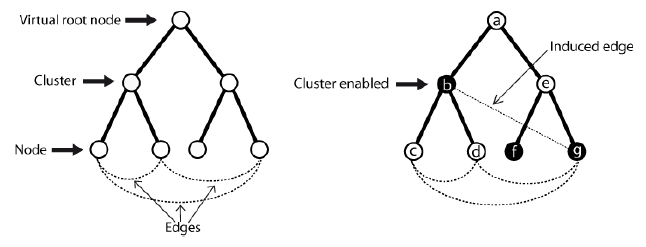
\includegraphics[width=10cm,keepaspectratio=true]{res/hierarchy.png}
  \caption{Graph tree with a virtual edge from a cluster to a leaf}
  \end{center}
\end{figure}

\paragraph{}
Two ways are available:
\begin{enumerate}
 \item Nodes can simply host other nodes and so on.
 \item Each node refers to a parent node id with the XML-attribute \begin{footnotesize}pid\end{footnotesize}.
\end{enumerate}

\lstset{ style=rnc }
\begin{lstlisting}[caption={Hierarchy Specification},label=hierarchyRNC]
# Extension Point
node-content &=
    attribute pid { id-type }?
  & element nodes { nodes-content }?
  & element edges { edges-content }?
\end{lstlisting}

The first style is preferred when the structure written is previously ordered. Sequential reading of this kind of GEXF is safe because no node reference is used. But in the case your program can't provide this, the second way allows writing (and then reading) nodes randomly, but linear reading is at your own risks.

\subsection{Sequential-safe Reading}

\lstset{ style=gexf }
\begin{lstlisting}[caption={First way},label=hierarchy1]
    <graph mode="static" defaultedgetype="directed">
        <nodes>
          <node id="a" label="Kevin Bacon">
            <nodes>
              <node id="b" label="God">
                <nodes>
                  <node id="c" label="human1"/>
                  <node id="d" label="human2"/>
                </nodes>
              </node>
              <node id="e" label="Me">
                <nodes>
                  <node id="f" label="frog1"/>
                  <node id="g" label="frog2"/>
                </nodes>
              </node>
            </nodes>
          </node>
        </nodes>
        <edges>
            <edge id="0" source="b" target="e" />
            <edge id="1" source="c" target="d" />
            <edge id="2" source="g" target="b" />
            <edge id="3" source="f" target="a" />
        </edges>
    </graph>
\end{lstlisting}

Note that edges are not necessarily written at the end:
\lstset{ style=gexf }
\begin{lstlisting}[caption={First way with edges inside clusters},label=hierarchy11]
    <graph mode="static" defaultedgetype="directed">
        <nodes>
          <node id="a" label="Kevin Bacon">
            <nodes>
              <node id="b" label="God">
                <nodes>
                  <node id="c" label="human1"/>
                  <node id="d" label="human2"/>
                </nodes>
                <edges>
                  <edge id="0" source="c" target="d" />
                </edges>
              </node>
              <node id="e" label="Me">
                <nodes>
                  <node id="f" label="frog1"/>
                  <node id="g" label="frog2"/>
                </nodes>
              </node>
            </nodes>
            <edges>
              <edge id="1" source="b" target="e" />
              <edge id="3" source="f" target="a" />
              <edge id="2" source="g" target="b" />
            </edges>
          </node>
        </nodes>
        <edges />
    </graph>
\end{lstlisting}

\subsection{Random Writing}

If you can't structurize your graph topology before writing a GEXF file, you may use the second style. Nodes sent to Gephi from a live data source, i.e. a web crawler, are written like this. Note that edges are always written randomly.

\lstset{ style=gexf }
\begin{lstlisting}[caption={Second way},label=hierarchy2]
<nodes>
  <node id="a" label="Kevin Bacon" />
  <node id="b" label="God" pid="a" />
  <node id="c" label="human1" pid="b" />
  <node id="d" label="human2" pid="b" />
  <node id="e" label="Me" pid="a" />
  <node id="f" label="frog1" pid="e" />
  <node id="g" label="frog2" pid="e" />
</nodes>
\end{lstlisting}

With using \begin{footnotesize}pid\end{footnotesize}, node order doesn't matter. An implementation should manage the case when a node reference (pid) is used before the node declaration. This listings could also be:

\lstset{ style=gexf }
\begin{lstlisting}[caption={Second way randomized},label=hierarchy22]
<nodes>
  <node id="g" label="frog2" pid="e" />
  <node id="a" label="Kevin Bacon" />
  <node id="c" label="human1" pid="b" />
  <node id="b" label="God" pid="a" />
  <node id="e" label="Me" pid="a" />
  <node id="d" label="human2" pid="b" />
  <node id="f" label="frog1" pid="e" />
</nodes>
\end{lstlisting}


\section{Advanced Concepts II: Phylogeny structure} \label{hierarchy}

Multiple parents can be adressed with the following syntax, where a and b are c's parents:
\lstset{ style=gexf }
\begin{lstlisting}[caption={Multiple parents},label=phylogeny1]
<nodes>
  <node id="a" label="cheese">
  <node id="b" label="cherry">
  <node id="c" label="cake">
    <parents>
      <parent for="a" />
      <parent for="b" />
    </parents>
  </node>
</nodes>
\end{lstlisting}

\lstset{ style=rnc }
\begin{lstlisting}[caption={Phylogeny Specification},label=phylogenyRNC]
# Extension Point
node-content &=
    element parents { parents-content }?

# New Point
parents-content =
    element parent { parent-content }*

# New Point
parent-content =
    attribute for { id-type }
\end{lstlisting}

\section{Advanced Concepts III: Dynamics} \label{dynamics}

As networks dynamics is a growing topic of research, GEXF format includes time support. Enable it by setting the \begin{footnotesize}mode\end{footnotesize} attribute of the graph to \textit{dynamic}.

\lstset{ style=gexf }
\begin{lstlisting}[caption={Dynamic Enabled!},label=dynamicEnabled]
<graph mode="dynamic">
  ...
</graph>
\end{lstlisting}

Time in GEXF is encoded in two ways, discrete or continuous.

Discrete, it is an \textit{integer} or a \textit{double}. Continuous, it is encoded as an international standard \textit{date} (yyyy-mm-dd) or a \textit{dateTime} defined by the corresponding \href{http://www.w3.org/TR/xmlschema-2/#dateTime}{XSD Datatype}. If omitted, the default type is \textit{double}. Use the the XML-attribute \begin{footnotesize}timeformat\end{footnotesize} of the graph element to explicitly declare the type.

Both network topology and data have a lifetime. The whole graph, each node, each edge and their respective data values may have time limits, beginning with an XML-attribute \begin{footnotesize}start\end{footnotesize} and ending with a \begin{footnotesize}end\end{footnotesize}. Omitting \begin{footnotesize}start\end{footnotesize} set the past of the thing to infinity, so as for \begin{footnotesize}end\end{footnotesize}. The file creator is responsible for the dates consistency.

Non-inclusive intervals are available as well: \begin{footnotesize}startopen\end{footnotesize} and \begin{footnotesize}endopen\end{footnotesize}. One can mix an inclusive and a non-inclusive boundary, but declaring both \begin{footnotesize}start\end{footnotesize} and \begin{footnotesize}startopen\end{footnotesize}, or both \begin{footnotesize}end\end{footnotesize} and \begin{footnotesize}endopen\end{footnotesize} for the same element is forbidden.

\subsection{Example}

\lstset{ style=gexf }
\begin{lstlisting}[caption={A (small) Dynamic Web Graph with continuous time},label=dynwebgraph]
<?xml version="1.0" encoding="UTF-8"?>
<gexf xmlns="http://www.gexf.net/1.2draft"
       xmlns:xsi="http://www.w3.org/2001/XMLSchema-instance"
       xsi:schemaLocation="http://www.gexf.net/1.2draft
                             http://www.gexf.net/1.2draft/gexf.xsd"
      version="1.2">
  <meta lastmodifieddate="2009-03-20">
    <creator>Gephi.org</creator>
    <description>A Web network changing over time</description>
  </meta>
  <graph mode="dynamic" defaultedgetype="directed" timeformat="date"
         start="2009-01-01" end="2009-03-20">
    <attributes class="node" mode="static">
      <attribute id="0" title="url" type="string"/>
      <attribute id="1" title="frog" type="boolean">
        <default>true</default>
      </attribute>
    </attributes>
    <attributes class="node" mode="dynamic">
      <attribute id="2" title="indegree" type="float"/>
    </attributes>
    <nodes>
      <node id="0" label="Gephi" start="2009-03-01">
        <attvalues>
          <attvalue for="0" value="http://gephi.org"/>
          <attvalue for="2" value="1"/>
        </attvalues>
      </node>
      <node id="1" label="Webatlas">
        <attvalues>
          <attvalue for="0" value="http://webatlas.fr"/>
          <attvalue for="2" value="1" end="2009-03-01"/>
          <attvalue for="2" value="2" start="2009-03-01" end="2009-03-10"/>
          <attvalue for="2" value="1" start="2009-03-11"/>
        </attvalues>
      </node>
      <node id="2" label="RTGI" end="2009-03-10">
        <attvalues>
          <attvalue for="0" value="http://rtgi.fr"/>
          <attvalue for="2" value="0" end="2009-03-01"/>
          <attvalue for="2" value="1" start="2009-03-01"/>
        </attvalues>
      </node>
      <node id="3" label="BarabasiLab">
        <attvalues>
          <attvalue for="0" value="http://barabasilab.com"/>
          <attvalue for="1" value="false"/>
          <attvalue for="2" value="0" end="2009-03-01"/>
          <attvalue for="2" value="1" start="2009-03-01"/>
        </attvalues>
      </node>
    </nodes>
    <edges>
      <edge id="0" source="0" target="1" start="2009-03-01"/>
      <edge id="1" source="0" target="2"
             start="2009-03-01" end="2009-03-10"/>
      <edge id="2" source="1" target="0" start="2009-03-01"/>
      <edge id="3" source="2" target="1" end="2009-03-10"/>
      <edge id="4" source="0" target="3" start="2009-03-01"/>
    </edges>
  </graph>
</gexf>
\end{lstlisting}

\subsection{Dynamic Topology}

Time limits declared for a graph element are optional, however they could save pre-importing computation. Time limits of edges must be consistent with the related nodes'ones.

The graph scope is defined as follow for a network from 2009-01-01 to 2009-03-20:

\lstset{ style=gexf }
\begin{lstlisting}[caption={Graph Scope Example}]
<graph mode="dynamic" start="2009-01-01" end="2009-03-20">
\end{lstlisting}

Each edge must declare time limits inside the join scope of \begin{footnotesize}source\end{footnotesize} and \begin{footnotesize}target\end{footnotesize}:
\begin{itemize}
 \item edge.start $\le$ (source.start and target.start)
 \item edge.end   $\ge$ (source.end   and target.end)
\end{itemize}

\lstset{ style=gexf }
\begin{lstlisting}[caption={Edge Scope Example}]
<nodes>
  <node id="0" label="Hello" start="2009-01-01" end="2009-02-01" />
  <node id="1" label="World" start="2009-01-15" end="2009-03-20" />
  ...
</nodes>
<edges>
  <edge id="0" source="0" target="1" start="2009-01-20" end="2009-02-01"/>
</edges>
\end{lstlisting}

Important: \begin{footnotesize}start\end{footnotesize} and \begin{footnotesize}end\end{footnotesize} values are inclusive, i.e. the following line is allowed:

\lstset{ style=gexf }
\begin{lstlisting}[caption={Smallest time scope}]
<edge id="0" source="0" target="1" start="2009-01-20" end="2009-01-20"/>
\end{lstlisting}

And of course the \begin{footnotesize}end\end{footnotesize} value must be later than the \begin{footnotesize}start\end{footnotesize} value. Using a non-inclusive \begin{footnotesize}endopen\end{footnotesize} value implies to keep it strictly greater than the \begin{footnotesize}start\end{footnotesize} value.

\paragraph{}
If a node or an edge exists only at some timeranges, we use the concept of spells. Spells are not provided for data values, which are only limited by one \begin{footnotesize}start\end{footnotesize} and one \begin{footnotesize}end\end{footnotesize}. Use the xml-element \begin{footnotesize}spells\end{footnotesize} for topology like this:

\lstset{ style=gexf }
\begin{lstlisting}[caption={Node with multiple spells}]
<gexf ...>
  ...
  <graph mode="dynamic" timeformat="date">
    <node id="0" label="Hello">
      <spells>
        <spell start="2009-01-01" end="2009-01-15" />
        <spell start="2009-01-30" end="2009-02-01" />
      </spells>
    </node>
    ...
  </graph>
</gexf>
\end{lstlisting}

If the xml-attributes \begin{footnotesize}start\end{footnotesize} and \begin{footnotesize}end\end{footnotesize} are used in node like before, they should be ignored by parsers: if spells are provided, only their content are taken into account. If no \begin{footnotesize}start\end{footnotesize} is provided, the spell begins with the network. If no \begin{footnotesize}end\end{footnotesize} is provided, the spell ends with the network. If two spells are covering a same period of time, parsers should consider them as a unique spell.

\lstset{ style=rnc }
\begin{lstlisting}[caption={Dynamic Topology Specification},label=dyntopoRNC]
# Extension Point
graph-content &=
    attribute timeformat { timeformat-type }?
  & (
      ( attribute start { time-type }?
      | attribute startopen { time-type }?)
      &
      ( attribute end { time-type }?
      & attribute endopen { time-type }?)
  )

# Extension Point
node-content &= (
      ( attribute start { time-type }?
      | attribute startopen { time-type }?)
      &
      ( attribute end { time-type }?
      & attribute endopen { time-type }?)
  )
  & element spells { spells-content }?

# Extension Point
edge-content &= (
      ( attribute start { time-type }?
      | attribute startopen { time-type }?)
      &
      ( attribute end { time-type }?
      & attribute endopen { time-type }?)
  )
  & element spells { spells-content }?
\end{lstlisting}

\paragraph{}
About the weight: dynamic weight can be used with the reserved \textit{title} "weight" in attributes. In dynamic mode, the static XML-attribute \textit{weight} should be ignored if the dynamic one is provided.

\subsection{Dynamic Data}

Node and edges data can take different values over time. Attributes must be declared as dynamic, allowing values to exist in during a time scope.

\subsubsection{Declaring Dynamic Attributes}

\lstset{ style=gexf }
\begin{lstlisting}[caption={Indegree may change over time!}]
<gexf ...>
  ...
  <graph mode="dynamic" defaultedgetype="directed">
    <attributes class="node" mode="dynamic">
      <attribute id="2" title="indegree" type="float"/>
      ...
    </attributes>
    ...
  </graph>
</gexf>
\end{lstlisting}

\lstset{ style=rnc }
\begin{lstlisting}[caption={Dynamic Attributes Specification},label=dyndataRNC]
# Extension Point
attributes-content &= (
      ( attribute start { time-type }?
      | attribute startopen { time-type }?)
      &
      ( attribute end { time-type }?
      & attribute endopen { time-type }?)
  )
\end{lstlisting}

\subsubsection{Defining Dynamic Values}

Attvalues have their scopes limited by the xml-attributes \begin{footnotesize}start\end{footnotesize} and \begin{footnotesize}end\end{footnotesize}.

\lstset{ style=gexf }
\begin{lstlisting}[caption={Data value changing over time}]
<node id="3" label="BarabasiLab">
  <attvalues>
    <attvalue for="2" value="0" start="2009-01-01" end="2009-03-01"/>
    <attvalue for="2" value="1" start="2009-03-02" end="2009-03-10"/>
  </attvalues>
</node>
\end{lstlisting}

\lstset{ style=gexf }
\begin{lstlisting}[caption={Using open and closed intervals}]
<node id="3" label="BarabasiLab">
  <attvalues>
    <attvalue for="2" value="15.0" start="2000" end="2005" />
          <attvalue for="2" value="20.0" startopen="2005" endopen="2010" />
          <attvalue for="2" value="25.0" start="2010" endopen="2015" />
  </attvalues>
</node>
\end{lstlisting}

\lstset{ style=rnc }
\begin{lstlisting}[caption={Dynamic Values Specification},label=dynvalRNC]
# Extension Point
attributes-content &= (
      ( attribute start { time-type }?
      | attribute startopen { time-type }?)
      &
      ( attribute end { time-type }?
      & attribute endopen { time-type }?)
  )
\end{lstlisting}

\subsubsection{Dynamic Values and Spells}

If an \begin{footnotesize}attvalue\end{footnotesize} is covering a period out of any spell, this period should be ignored by parsers. In the following example, the day 2009-01-03 is ignored:

\lstset{ style=gexf }
\begin{lstlisting}[caption={Spells and attvalues}]
<gexf ...>
  ...
  <graph mode="dynamic">
    <node id="0" label="Hello">
      <attvalues>
        <attvalue for="0" value="1" start="2009-01-01" end="2009-01-05"/>
      </attvalues>
      <spells>
        <spell start="2009-01-01" end="2009-01-02" />
        <spell start="2009-01-04" end="2009-01-05" />
      </spells>
    </node>
    ...
  </graph>
</gexf>
\end{lstlisting}

\paragraph{}
If a value 'B' is declared after a value 'A' of the same attribute and overlaps it, then 'A' is forced to end at 'B' start. In the following example, 'A' will effectively end at 2009-03-03, and the value at 2009-03-03 is 'B':

\lstset{ style=gexf }
\begin{lstlisting}[caption={Value overlapping}]
<node id="0" label="Hello">
  <attvalues>
    <attvalue for="0" value="A" start="2009-03-01" end="2009-03-05"/>
    <attvalue for="0" value="B" start="2009-03-03" end="2009-03-10"/>
  </attvalues>
</node>
\end{lstlisting}

One of the consequences of this rule is the right to end 'A' exactly with the 'B' start. Attribute '0' takes then the value 'B' at 2009-03-01.

\lstset{ style=gexf }
\begin{lstlisting}[caption={Value transition}]
<node id="0" label="Hello">
  <attvalues>
    <attvalue for="0" value="A" end="2009-03-01"/>
    <attvalue for="0" value="B" start="2009-03-01"/>
  </attvalues>
</node>
\end{lstlisting}

\paragraph{}
While each data value is encoded in one piece of time, spells can cut them into more pieces. In the following example, a node exists from the beginning of the graph to 2009-03-01, and re-appears from 2009-03-05 to 2009-03-10. The data values will then fit inside these scopes even if they initially have a larger scope. Value 'A' of attribute '2' will be effective in 2009-03-01 (dates are inclusive), and from 2009-03-05 to 2009-03-10.

\lstset{ style=gexf }
\begin{lstlisting}[caption={Spells}]
<node id="2" label="RTGI">
  <attvalues>
    <attvalue for="0" value="http://rtgi.fr"/>
    <attvalue for="2" value="X" end="2009-02-28"/>
    <attvalue for="2" value="A" start="2009-03-01"/>
  </attvalues>
  <spells>
    <spell end="2009-03-01">
    <spell start="2009-03-05" end="2009-03-10">
  </spells>
</node>
\end{lstlisting}

\lstset{ style=rnc }
\begin{lstlisting}[caption={Spells Specification},label=dynspellsRNC]
# New Point
spells-content =
    element spell { spell-content }+

# New Point
spell-content = (
      ( attribute start { time-type }?
      | attribute startopen { time-type }?)
      &
      ( attribute end { time-type }?
      & attribute endopen { time-type }?)
  )
\end{lstlisting}

\section{Advanced Concepts IV: Extending GEXF} \label{extendgexf}

GEXF is designed to be easily extensible. Additional namespaces are defined by an XML Schema. The default namespace is always the gexf namespace. Gephi team actually provides a module for storing visualization data called \textit{viz}.

\subsection{VIZ module} \label{viz}

Using the visualization module must be declared by adding the XML Attribute \begin{footnotesize}xmlns:viz="http://www.gexf.net/1.2draft/viz"\end{footnotesize} to the document namespaces. The \begin{footnotesize}xsi:schemaLocation\end{footnotesize} attribute includes the XML-Schema declaration of the VIZ module. The RelaxNG Compact specification is available in \href{http://www.gexf.net/1.2draft/viz.rnc}{viz.rnc}, and independent XSD declaration in \href{http://www.gexf.net/1.2draft/viz.xsd}{viz.xsd}.

Color, position, size and shape are stored as attributes.

\paragraph{}
These elements are compatible with spells and intervals defined in previous section.

\subsubsection{Node Example}

The following gexf contains a node having a color, a position, a shape and a specified size.

\lstset{ style=gexf }
\begin{lstlisting}[caption={VIZ Attributes},label=vizattr]
<gexf xmlns="http://www.gexf.net/1.2draft"
      xmlns:viz="http://www.gexf.net/1.2draft/viz">
...
  <node ... >
    <viz:color r="239" g="173" b="66" a="0.5"/>
    <viz:position x="15.783598" y="40.109245" z="0.0"/>
    <viz:size value="2.0375757"/>
    <viz:shape value="disc"/>
  </node>
...
</gexf>
\end{lstlisting}

\subsubsection{Edge Example}

The following gexf contains an edge having a color, a thickness and a shape.

\lstset{ style=gexf }
\begin{lstlisting}[caption={VIZ Attributes},label=vizattr]
<gexf xmlns="http://www.gexf.net/1.2draft"
      xmlns:viz="http://www.gexf.net/1.2draft/viz">
...
  <edge ... >
    <viz:color r="157" g="213" b="78"/>
    <viz:thickness value="5.124"/>
    <viz:shape value="solid"/>
  </edge>
...
</gexf>
\end{lstlisting}

\subsubsection{Colors}

Colors are defined by the \href{http://en.wikipedia.org/wiki/RGBA}{RGBA color model}. Each XML-attribute value \begin{footnotesize}r\end{footnotesize}, \begin{footnotesize}g\end{footnotesize} or \begin{footnotesize}b\end{footnotesize} is hence an integer from 0 to 255, and the alpha value \begin{footnotesize}a\end{footnotesize} is a float from 0.0 to 1.0.

\lstset{ style=gexf }
\begin{lstlisting}[caption={VIZ Color Declaration},label=vizcolor]
<viz:color r="239" g="173" b="66" a="0.5"/>
\end{lstlisting}

\lstset{ style=rnc }
\begin{lstlisting}[caption={Color Specification},label=colorRNC]
# Extension Point
node-content &=
    element color { color-content }?

# New Point
color-content =
    attribute r { color-channel }
  & attribute g { color-channel }
  & attribute b { color-channel }
  & attribute a { alpha-channel }?

# Datatypes

color-channel =
    xsd:nonNegativeInteger { maxInclusive = "255" }

alpha-channel = [ a:defaultValue = "1.0" ]
    xsd:float { minInclusive = "0.0" maxInclusive = "1.0" }
\end{lstlisting}

\subsubsection{Position}

Space positions are set in three dimensions called \begin{footnotesize}x\end{footnotesize}, \begin{footnotesize}y\end{footnotesize} and \begin{footnotesize}z\end{footnotesize}. Note that Gephi associates \begin{footnotesize}z\end{footnotesize} as the height, and most of spatialization algorithms only use \begin{footnotesize}x\end{footnotesize} and \begin{footnotesize}y\end{footnotesize}. They are floats.

\lstset{ style=gexf }
\begin{lstlisting}[caption={VIZ Position Declaration},label=vizposition]
<viz:position x="15.783598" y="40.109245" z="0.0"/>
\end{lstlisting}

\lstset{ style=rnc }
\begin{lstlisting}[caption={Position Specification},label=positionRNC]
# Extension Point
node-content &=
  element position { position-content }?

# New Point
position-content =
    attribute x { space-point }
  & attribute y { space-point }
  & attribute z { space-point }

# Datatype
space-point =
    xsd:float
\end{lstlisting}

\subsubsection{Size}

Node size is a scale. It is set to \textit{1.0} by default and is a non-negative float. Network viz softwares assume that an object representing a node of size \textit{2.0} is twice bigger as one of \textit{1.0}.

\lstset{ style=gexf }
\begin{lstlisting}[caption={VIZ Size Declaration},label=vizsize]
<viz:size value="2.0375757"/>
\end{lstlisting}

\lstset{ style=rnc }
\begin{lstlisting}[caption={Size Specification},label=sizeRNC]
# Extension Point
node-content &=
  element size { size-content }?

# New Point
size-content =
    attribute value { size-type }

# Datatype
size-type = [ a:defaultValue = "1.0" ]
    xsd:float { minInclusive = "0.0"}
\end{lstlisting}

\subsubsection{Thickness}

Edge thickness is a scale. It is set to \textit{1.0} by default and is a non-negative float. Network viz softwares assume that an object representing an edge of thickness \textit{2.0} is twice bigger as one of \textit{1.0}.

\lstset{ style=gexf }
\begin{lstlisting}[caption={VIZ Thickness Declaration},label=vizthickness]
<viz:size value="2.0375757"/>
\end{lstlisting}

\lstset{ style=rnc }
\begin{lstlisting}[caption={Thickness Specification},label=thicknessRNC]
# Extension Point
edge-content &=
  element thickness { thickness-content }?

# New Point
thickness-content =
    attribute value { thickness-type }

# Datatype
thickness-type = [ a:defaultValue = "1.0" ]
    xsd:float { minInclusive = "0.0"}
\end{lstlisting}

\subsubsection{Node Shape}

Default node is shaped as a disc. Four shapes are proposed: \textit{disc}, \textit{square}, \textit{triangle} and \textit{diamond}. Images require an additional xml-attribute to set their location: \begin{footnotesize}uri\end{footnotesize}.

\lstset{ style=rnc }
\begin{lstlisting}[caption={Node Shape Specification},label=nshapeRNC]
# Extension Point
node-content &=
  element shape { node-shape-content }?

# New Point
node-shape-content =
    attribute value { node-shape-type }
   & attribute uri { xsd:anyURI }?

# Datatype
node-shape-type =  [ a:defaultValue = "disc" ]
    string "disc" |
    string "square" |
    string "triangle" |
    string "diamond" |
    string "image"
\end{lstlisting}

\lstset{ style=gexf }
\begin{lstlisting}[caption={Image Declaration},label=vizimage]
<viz:shape value="image" uri="http://my.image.us/blah.jpg"/>
\end{lstlisting}

\subsubsection{Edge Shape}

Default edge is shaped as solid. Four shapes are proposed: \textit{solid}, \textit{dotted}, \textit{dashed} and \textit{double}.

\lstset{ style=rnc }
\begin{lstlisting}[caption={Edge Shape Specification},label=eshapeRNC]
# Extension Point
edge-content &=
  element shape { edge-shape-content }?

# New Point
edge-shape-content =
    attribute value { edge-shape-type }

# Datatype
edge-shape-type =  [ a:defaultValue = "solid" ]
    string "solid" |
    string "dotted" |
    string "dashed" |
    string "double"
\end{lstlisting}

\section{Advices: Parser optimization} \label{advices}

This section provides some good tips to write parser-friendly files.
\begin{itemize}
 \item Always place the edges after the nodes, as it is mandatory since version 1.2. Some parsers, depending on their implementation, may reject an edge if its linked nodes haven't been declared before, due to conceptual or data integrity reason.
 \item Use the \textit{count} XML-attribute in \textit{nodes} and \textit{edges} declaration: the parser will know how much memory it should allocate, and will speed up the file reading. Note that count only refers to direct children, not the whole sub-graph!
 \item Prefer \textit{liststring} to \textit{string} attributes if you can. A smart parser will store the strings in one place, and just set pointers to them from the related nodes/edges.
 \item Identifiers may be interpreted as integers if you only use numbers. We encourage this practice, as an integer takes much less size in memory than an equivalent string. Tell the parser to optimize IDs storage by filling the optional graph XML-attribute called \textit{idtype} with “string“ or “integer“.
\end{itemize}

\section{Web Services} \label{ws}

The content-type for serving GEXF files via HTTP/REST is \textit{application/gexf+xml}.

\section{Changelog} \label{changelog}

This document has been edited on:
\begin{itemize}
\item 28 March 2012 -- Add open interval example in section Defining Dynamic Values
\item 29 Nov 2010 -- Initial release
\end{itemize}

\printindex

\end{document}
